\newpage
\subsection{Attività preliminari di avvio ed analisi dei requisiti}
	\subsubsection{Prospetto orario}
	La distribuzione oraria della fase di Analisi è la seguente:
	
		\begin{table}[!htbp]
			\centering
			\renewcommand{\arraystretch}{2} 
			\rowcolors{2}{gray!25}{white}
			\begin{tabular}{|l c c c c c c|c| }
				\rowcolor{orange!50}
				\hline
				\multicolumn{8}{|c|}{\textbf{Suddivisione delle ore nei vari ruoli}}\\
				\hline
				\textbf{Nominativo} & RES 	& AMM 	& ANA 	& PRO 	& PRG 	& VER 	& \textbf{Totale} \\
				\hline
				\mat 				& -		& 6		& 10	& -		& -		& 2		& 18\\
				\hline
				\pie 				& 12 	& -		& 6		& -		& - 	& -		& 18\\
				\hline
				\mic  				& -		& -		& 6		& -		& -		& 12	& 18\\
				\hline
				\mar  				& -		& 12	& 2		& -		& - 	& 4 	& 18\\
				\hline
				\daG  				& 6		& -		& 12	& -		& - 	& -		& 18\\
				\hline
				\daL 				& -		& 3		& 11	& -		& -		& 4		& 18\\
				\hline
				\gia 				& -		& 6		& -		& -		& -		& 12& 18\\
				\hline
			\end{tabular}
			\caption{Suddivisione ore del periodo di Analisi}
		\end{table}
	Di seguito rappresentata anche in un grafico:
		\begin{figure}[!htbp]
			\centering
			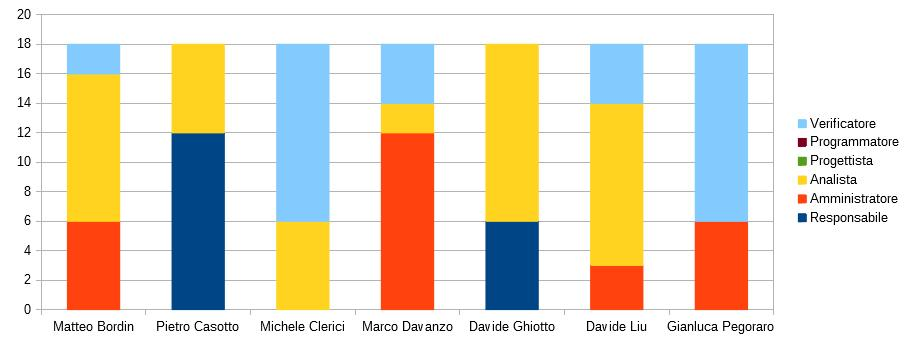
\includegraphics[scale=0.7]{preventivo/grafico_prima_parte.jpg}
			\caption{Grafico suddivisione oraria nel periodo di Analisi}
		\end{figure}
	\newpage
	\subsubsection{Conteggio ore}
		La distribuzione delle ore nei vari ruoli nella fase di Analisi è la seguente:
		
		\begin{table}[!htbp]
			\centering
			\renewcommand{\arraystretch}{1.8} 
			\rowcolors{2}{gray!25}{white}
			\begin{tabular}{| c c c|}
				\rowcolor{orange!50}
				\hline
				\multicolumn{3}{|c|}{\textbf{Suddivisione delle ore nei vari ruoli}}\\
				\hline
				\textbf{Ruolo} 			& Ore 	& Costo\\
				\hline
				\textbf{Responsabile}	& 18 	& 540\\
				\hline
				\textbf{Amministratore}	& 27 	& 540\\
				\hline
				\textbf{Analista}		& 47 	& 1175\\
				\hline
				\textbf{Progettista}	& 0 	& 0\\
				\hline
				\textbf{Programmatore}	& 0 	& 0\\
				\hline
				\textbf{Verificatore} 	& 34 	& 510\\
				\hline
				\textbf{Totale} 		& 126	& 2768\\
				\hline 
			\end{tabular}
			\caption{Ore e costi totali del periodo di Analisi}
		\end{table}
		\newpage
		Di seguito rappresentata anche in un grafico:
		\begin{figure}[!htbp]
			\centering
			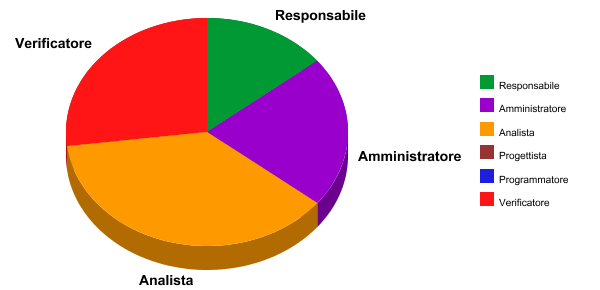
\includegraphics[scale=1]{preventivo/torta_prima_parte.png}
			\caption{Grafico suddivisione ruoli nel periodo di Analisi}
		\end{figure}
\clearpage
